\documentclass[11pt,a4paper]{article}
\usepackage[utf8]{inputenc}
\usepackage[margin=1in]{geometry}
\setlength{\headheight}{14pt}
\usepackage{graphicx}
\usepackage{amsmath,amssymb}
\usepackage{booktabs}
\usepackage{array}
\usepackage{hyperref}
\usepackage{float}
\usepackage{caption}
\usepackage{subcaption}
\usepackage{fancyhdr}
\usepackage{titlesec}
\usepackage{xcolor}

% Custom Colors
\definecolor{primary}{RGB}{0, 51, 102}
\definecolor{secondary}{RGB}{70, 130, 180}

\hypersetup{
    colorlinks=true,
    linkcolor=primary,
    citecolor=primary,
    urlcolor=secondary
}

% Header and Footer setup
\pagestyle{fancy}
\fancyhf{}
\rhead{\textcolor{primary}{\textbf{EDC Laboratory --- Experiment 1}}}
\lhead{\textcolor{primary}{\textbf{EE25BTECH11056 \& EE25BTECH11049}}}
\rfoot{Page \thepage}

\titleformat{\section}{\large\bfseries\color{primary}}{\thesection.}{0.5em}{}
\titleformat{\subsection}{\normalfont\bfseries\color{secondary}}{\thesubsection}{0.5em}{}

\begin{document}

% Title Page / Header Block
\begin{center}
    {\LARGE \textbf{\color{primary} DEPARTMENT OF ELECTRICAL ENGINEERING}}\\[0.2cm]
    {\large \textbf{Electronic Devices \& Circuits Laboratory (EDC LAB)}}\\[0.5cm]
    \rule{\linewidth}{1pt}\\[0.4cm]
    {\Large \textbf{EXPERIMENT 1: V--I Characteristics of PN Junction \& Zener Diodes, and Study of Clipper \& Clamper Circuits}}\\[0.4cm]
    \rule{\linewidth}{1pt}\\[0.6cm]
    
    \begin{tabular}{ll}
        \textbf{Prepared By:} & Suraj.N (EE25BTECH11056) \\
                             & Sai Krishna Bakki (EE25BTECH11049) \\
        \textbf{Course:} & Electronic Devices \& Circuits Lab \\
        \textbf{Date:} & \today
    \end{tabular}
\end{center}

\vspace{0.5cm}

\section{Aim}
\begin{enumerate}
    \item To plot the forward- and reverse-bias $V$--$I$ characteristics of a PN junction diode and determine its cut-in voltage ($V_\gamma$), static forward resistance ($R_{DC}$), dynamic forward resistance ($r_d$), and reverse saturation current ($I_s$).
    \item To plot the forward- and reverse-bias $V$--$I$ characteristics of a Zener diode (1N4733A) and determine its Zener breakdown voltage ($V_Z$) and Zener resistance ($R_Z$).
    \item To design, simulate, and test positive, negative, and biased (two-level) diode clipper circuits and observe their clipping levels.
    \item To design, simulate, and test positive and negative diode clamper circuits and measure the resulting DC voltage shift.
\end{enumerate}

\section{Apparatus and Software Tools Required}
\begin{table}[H]
\centering
\caption{Equipment and Components Specifications}
\begin{tabular}{cllc}
\toprule
\textbf{S.No.} & \textbf{Component / Equipment} & \textbf{Specification} & \textbf{Quantity} \\
\midrule
1 & PN Junction Diode & 1N4007 / 1N4148 & 1 \\
2 & Zener Diode & 1N4733A ($V_Z = 5.1\text{ V}, 1\text{ W}$) & 1 \\
3 & Resistors & $1\text{ k}\Omega$, $10\text{ k}\Omega$ & As required \\
4 & Capacitor & $0.1\text{ }\mu\text{F}$ & 1 \\
5 & DC Voltage Sources & $0$--$30\text{ V}$ Variable, $+1\text{ V}$, $-1\text{ V}$ Reference & As required \\
6 & Function Generator / AC Source & $1\text{ kHz}$ Sine wave, $4\text{ V}_{pp}$ & 1 \\
7 & Simulation Software & LTspice & -- \\
\bottomrule
\end{tabular}
\end{table}

\section{Part A: PN Junction Diode Characteristics}

\subsection{Theoretical Background}
A PN junction diode exhibits non-linear current-voltage characteristics described by the Shockley diode equation:
\begin{equation}
I = I_s \left( e^{\frac{V}{\eta V_T}} - 1 \right)
\end{equation}
where $I_s$ is the reverse saturation current, $V_T = \frac{k T}{q}$ is the thermal voltage ($\approx 26\text{ mV}$ at room temperature), and $\eta$ is the ideality factor.
\begin{itemize}
    \item \textbf{Forward Bias:} When anode is positive relative to cathode, the barrier potential is reduced. Below the cut-in voltage ($V_\gamma \approx 0.6\text{--}0.7\text{ V}$ for Silicon), current is negligible. Above $V_\gamma$, current increases exponentially.
    \item \textbf{Reverse Bias:} When cathode is positive relative to anode, the barrier height increases, allowing only a minute reverse saturation current $I_s$ to flow until reverse breakdown occurs.
\end{itemize}

\subsection{Circuit Diagrams and Simulation Waveforms}

\subsubsection{PN Junction Diode -- Forward Bias}
The forward bias circuit consists of a $1\text{ k}\Omega$ current-limiting resistor and a PN diode. The DC voltage supply is swept from $0\text{ V}$ upward.

\begin{figure}[H]
    \centering
    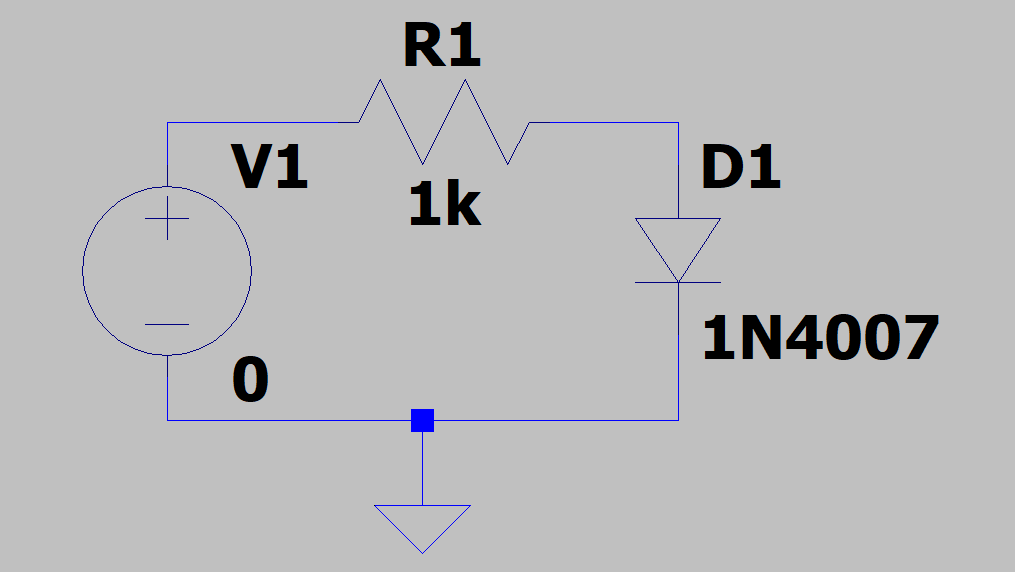
\includegraphics[width=0.55\textwidth]{EXP_1/DIODE_FORWARD/circuit.png}
    \caption{PN Junction Diode Forward Bias Circuit Schematic.}
    \label{fig:diode_fwd_circuit}
\end{figure}

\begin{figure}[H]
    \centering
    \begin{subfigure}[b]{0.48\textwidth}
        \centering
        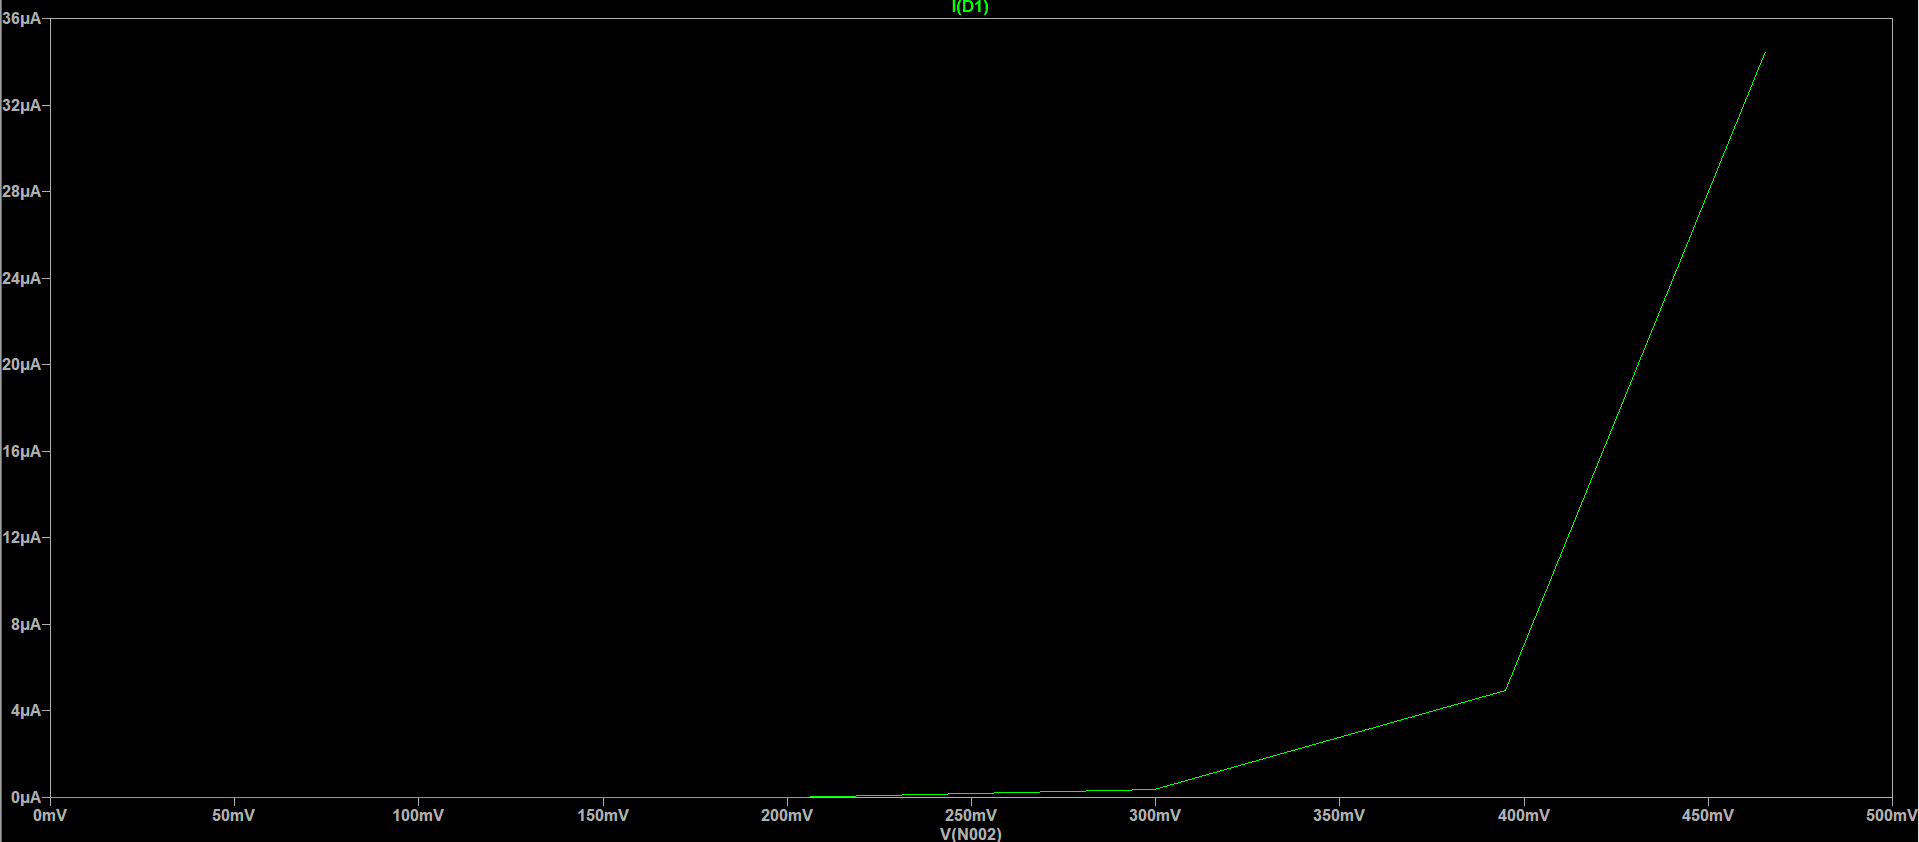
\includegraphics[width=\textwidth]{EXP_1/DIODE_FORWARD/0-0.5v.png}
        \caption{Low Voltage Sweep ($0\text{ V}$ to $0.5\text{ V}$)}
    \end{subfigure}
    \hfill
    \begin{subfigure}[b]{0.48\textwidth}
        \centering
        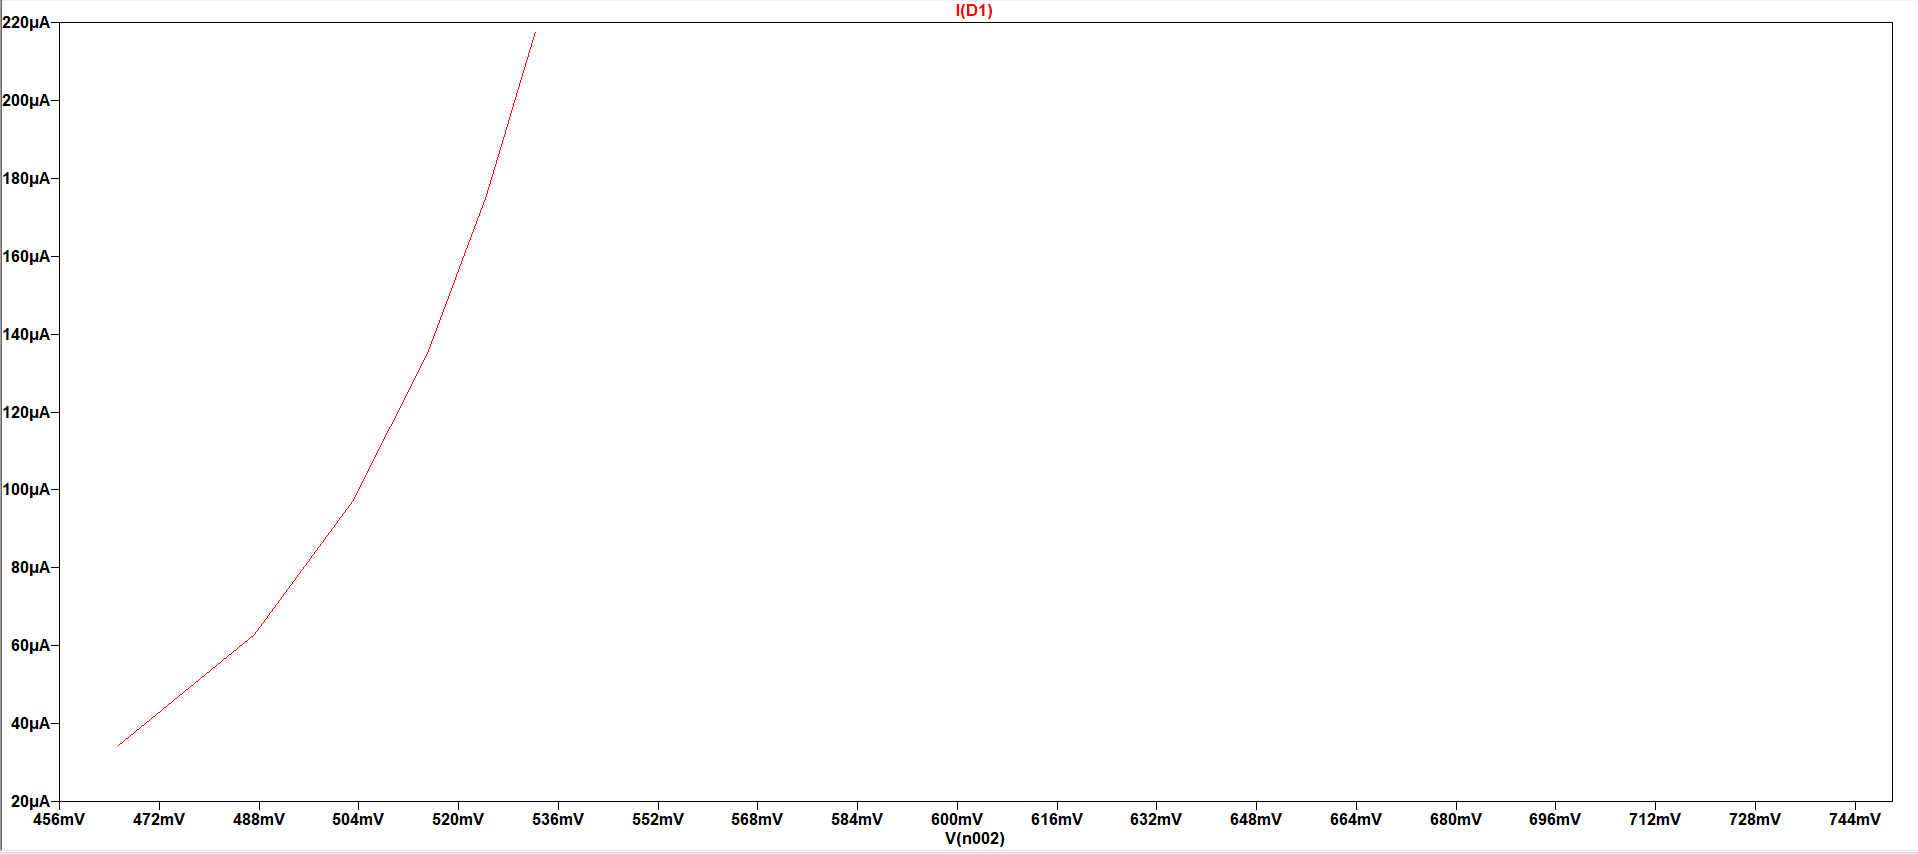
\includegraphics[width=\textwidth]{EXP_1/DIODE_FORWARD/0.5-0.75v.png}
        \caption{Knee Region Sweep ($0.5\text{ V}$ to $0.75\text{ V}$)}
    \end{subfigure}
    \caption{PN Diode Forward $V$--$I$ Characteristics Simulation Plots.}
    \label{fig:diode_fwd_sim}
\end{figure}

\subsubsection{PN Junction Diode -- Reverse Bias}
The reverse bias circuit reverses the diode polarity to measure the reverse saturation current across a $0\text{--}30\text{ V}$ sweep.

\begin{figure}[H]
    \centering
    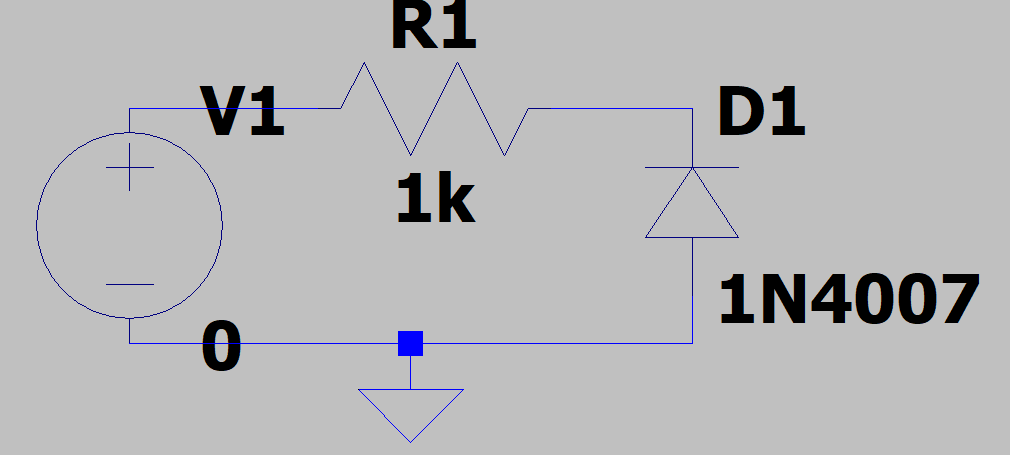
\includegraphics[width=0.55\textwidth]{EXP_1/DIODE_REVERSE/circuit.png}
    \caption{PN Junction Diode Reverse Bias Circuit Schematic.}
    \label{fig:diode_rev_circuit}
\end{figure}

\begin{figure}[H]
    \centering
    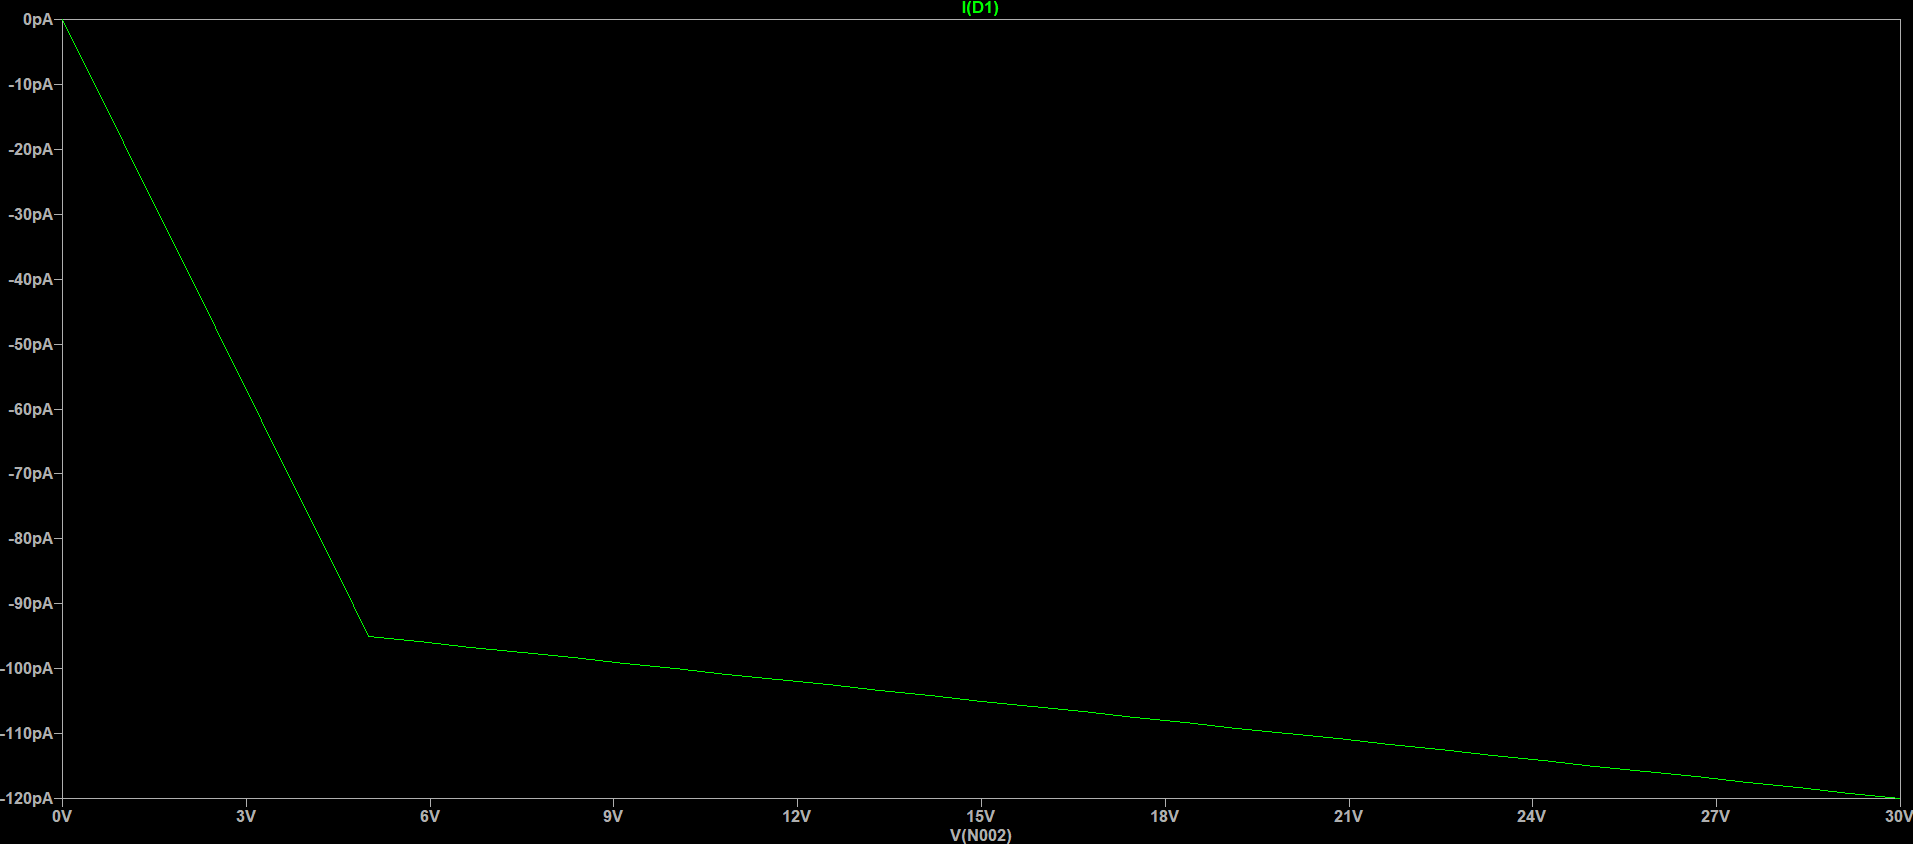
\includegraphics[width=0.65\textwidth]{EXP_1/DIODE_REVERSE/0-30v.png}
    \caption{PN Diode Reverse Characteristic ($0\text{ V}$ to $30\text{ V}$).}
    \label{fig:diode_rev_sim}
\end{figure}

\newpage
\section{Part B: Zener Diode Characteristics}

\subsection{Theoretical Background}
A Zener diode is designed to operate safely in the reverse breakdown region. When reverse-biased beyond the Zener breakdown voltage ($V_Z$), the voltage across the diode remains virtually constant over a wide range of currents. In forward bias, it behaves like an ordinary PN junction diode.

\subsection{Circuit Diagrams and Simulation Waveforms}

\subsubsection{Zener Diode -- Forward Bias}
\begin{figure}[H]
    \centering
    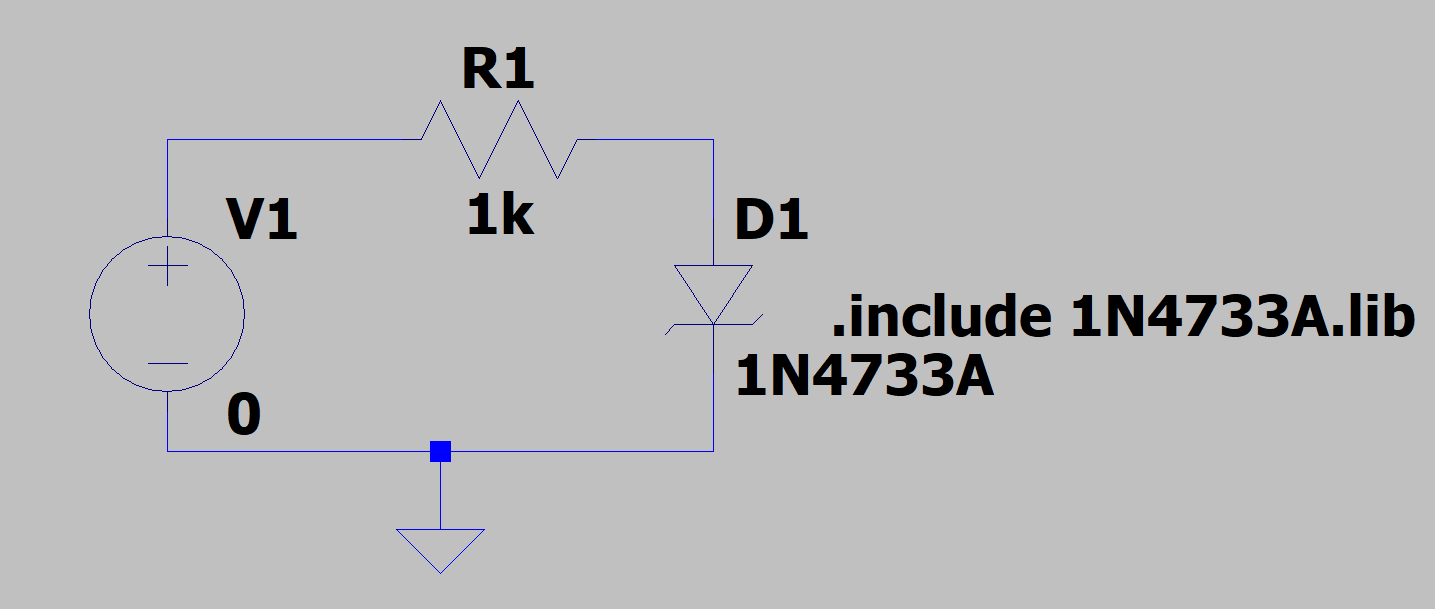
\includegraphics[width=0.55\textwidth]{EXP_1/ZENER_FORWARD/circuit.png}
    \caption{Zener Diode Forward Bias Circuit Schematic.}
    \label{fig:zener_fwd_circuit}
\end{figure}

\begin{figure}[H]
    \centering
    \begin{subfigure}[b]{0.48\textwidth}
        \centering
        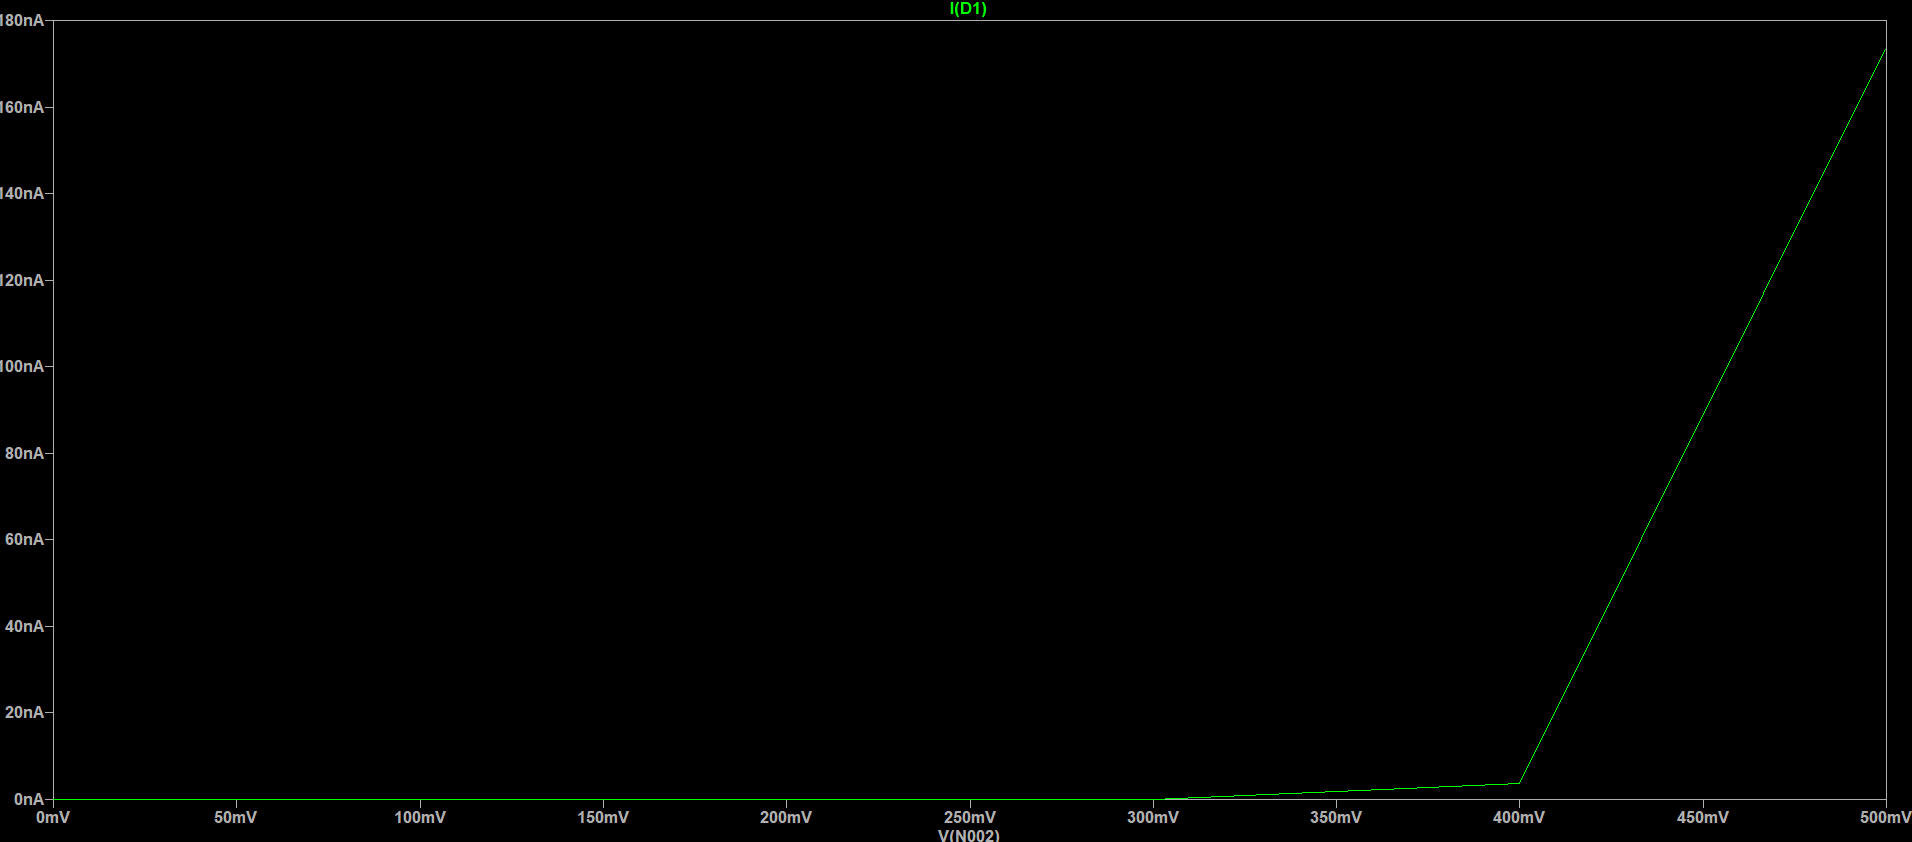
\includegraphics[width=\textwidth]{EXP_1/ZENER_FORWARD/0-0.5v.png}
        \caption{Sub-knee Voltage Region ($0\text{ V}$ to $0.5\text{ V}$)}
    \end{subfigure}
    \hfill
    \begin{subfigure}[b]{0.48\textwidth}
        \centering
        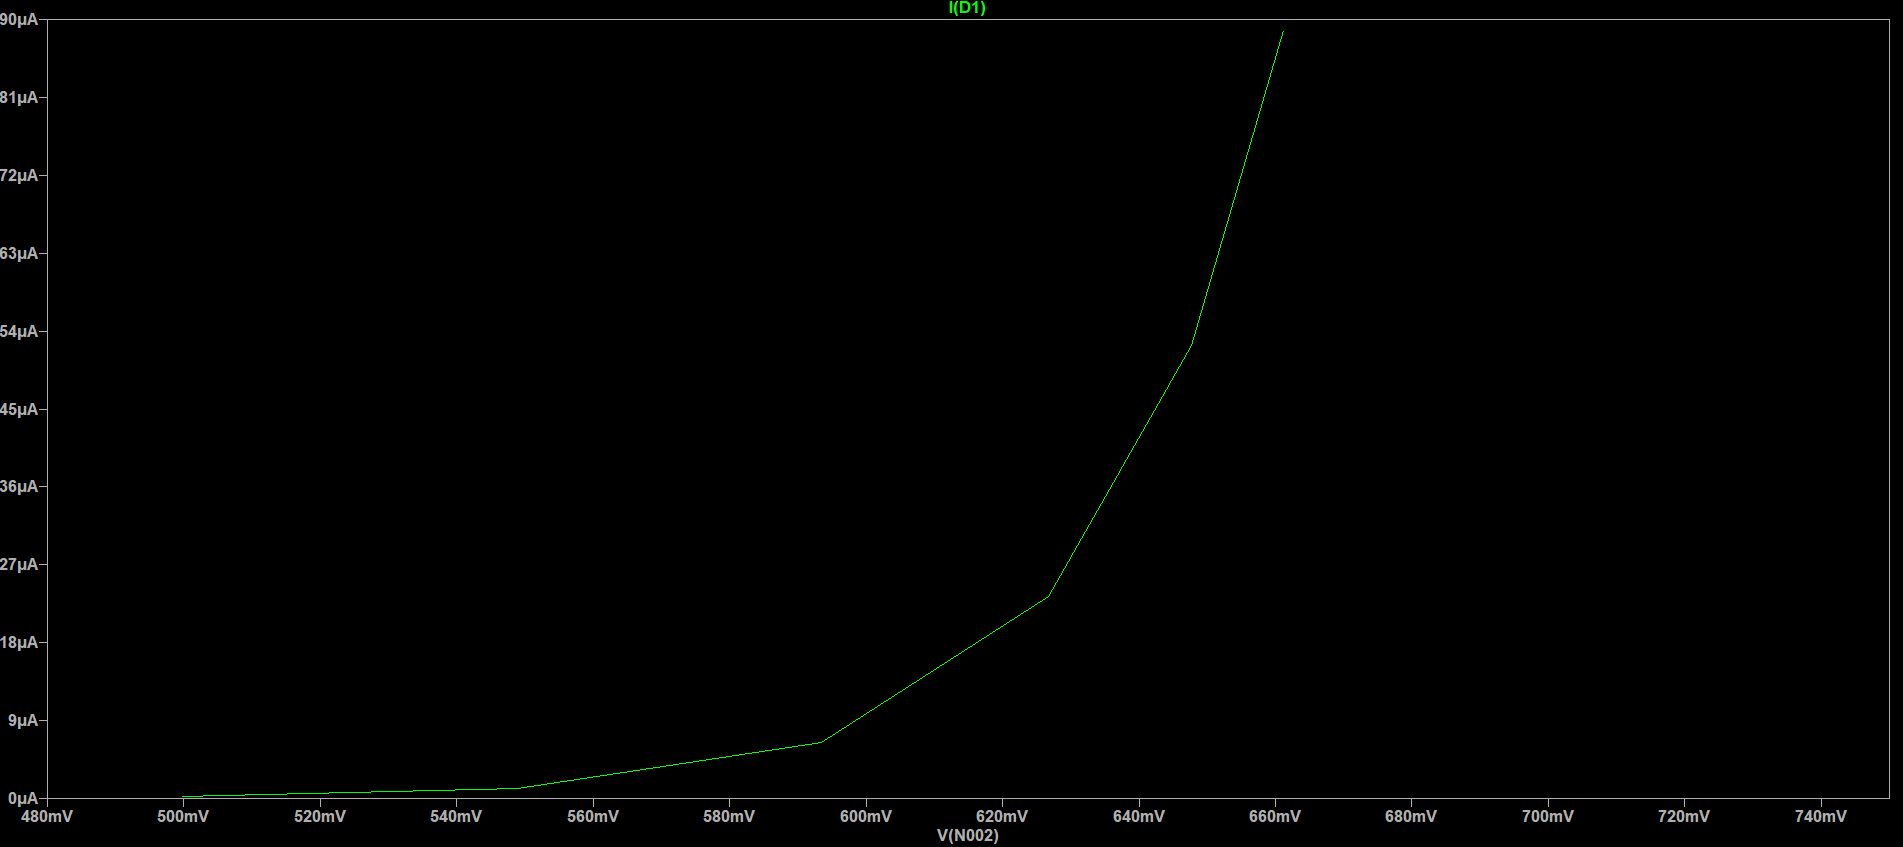
\includegraphics[width=\textwidth]{EXP_1/ZENER_FORWARD/0.5-0.75.png}
        \caption{Forward Conduction Region ($0.5\text{ V}$ to $0.75\text{ V}$)}
    \end{subfigure}
    \caption{Zener Diode Forward Bias Simulation Plots.}
    \label{fig:zener_fwd_sim}
\end{figure}

\subsubsection{Zener Diode -- Reverse Bias and Breakdown}
\begin{figure}[H]
    \centering
    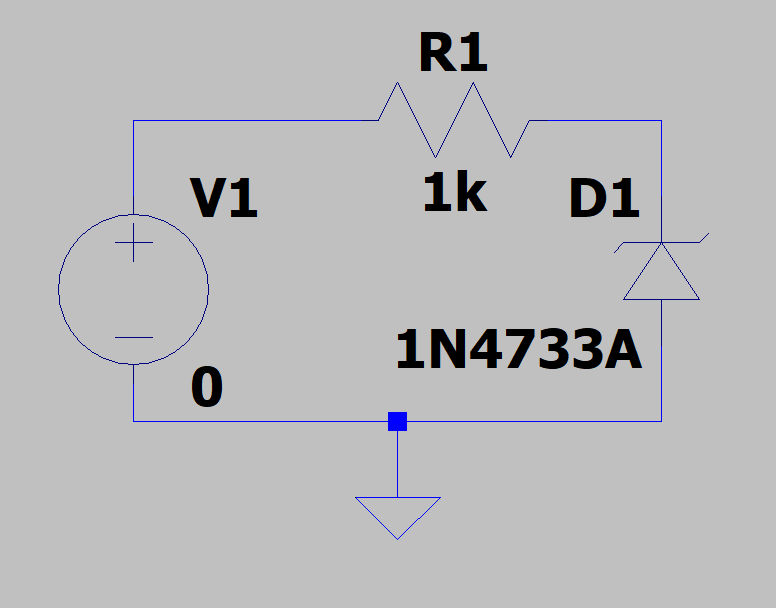
\includegraphics[width=0.55\textwidth]{EXP_1/ZENER_REVERSE/circuit.png}
    \caption{Zener Diode Reverse Bias Circuit Schematic.}
    \label{fig:zener_rev_circuit}
\end{figure}

\begin{figure}[H]
    \centering
    \begin{subfigure}[b]{0.32\textwidth}
        \centering
        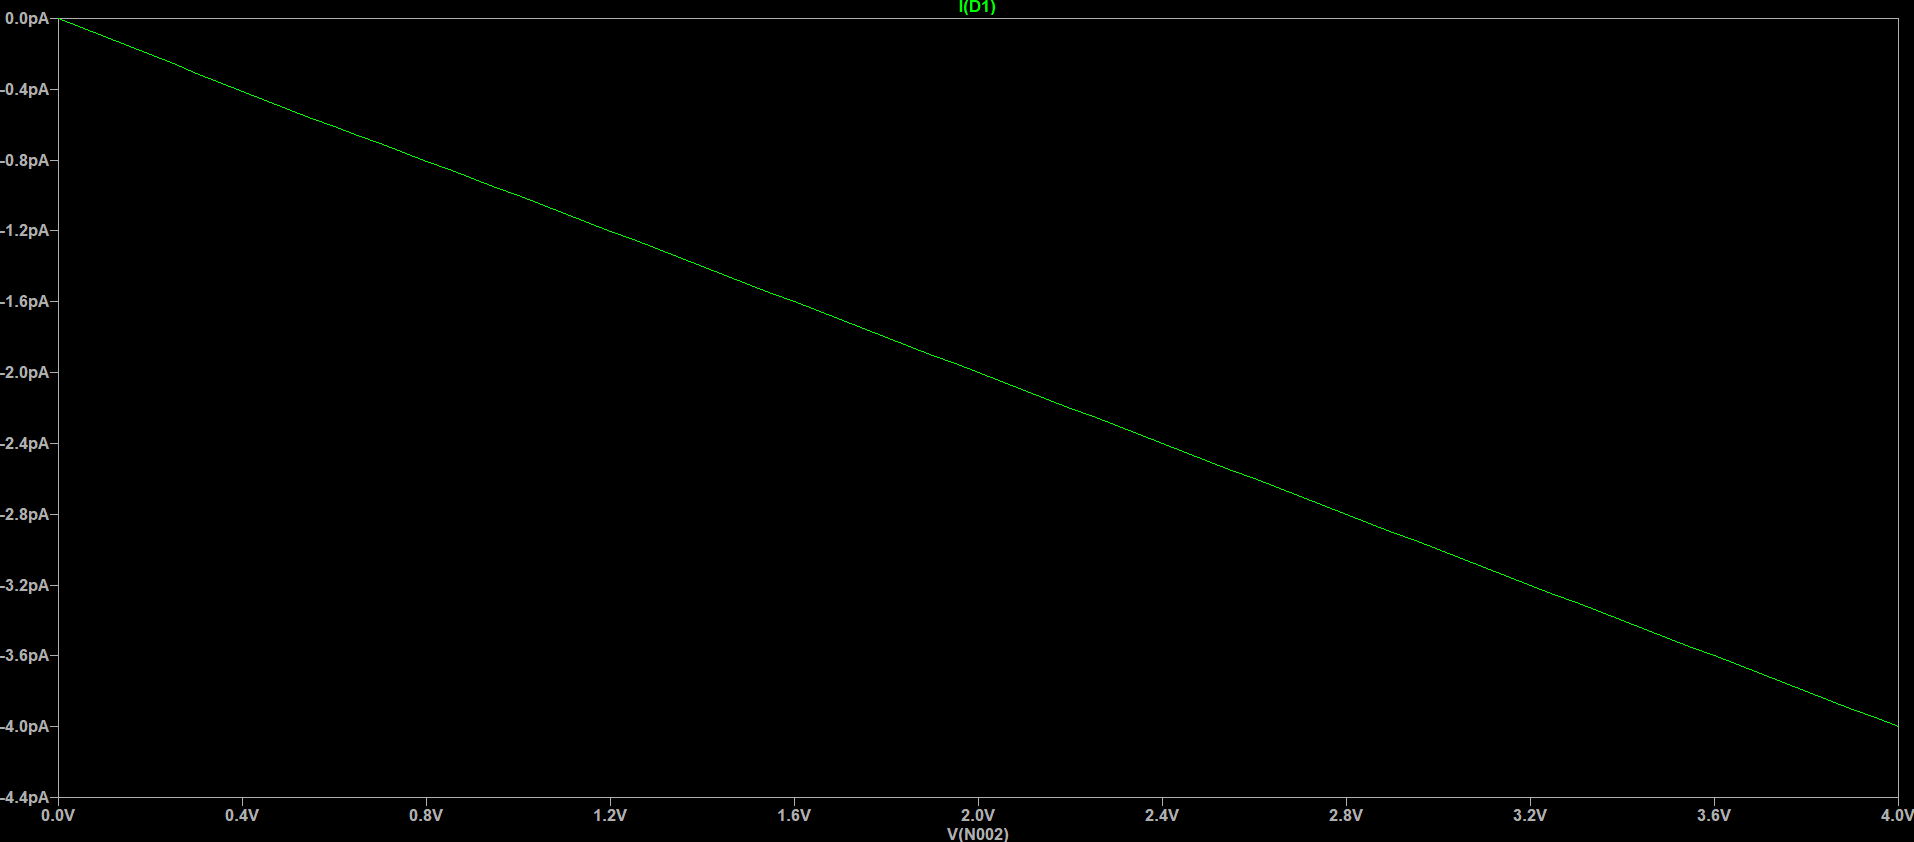
\includegraphics[width=\textwidth]{EXP_1/ZENER_REVERSE/0-4v.png}
        \caption{Pre-breakdown ($0\text{ V}$ to $4\text{ V}$)}
    \end{subfigure}
    \hfill
    \begin{subfigure}[b]{0.32\textwidth}
        \centering
        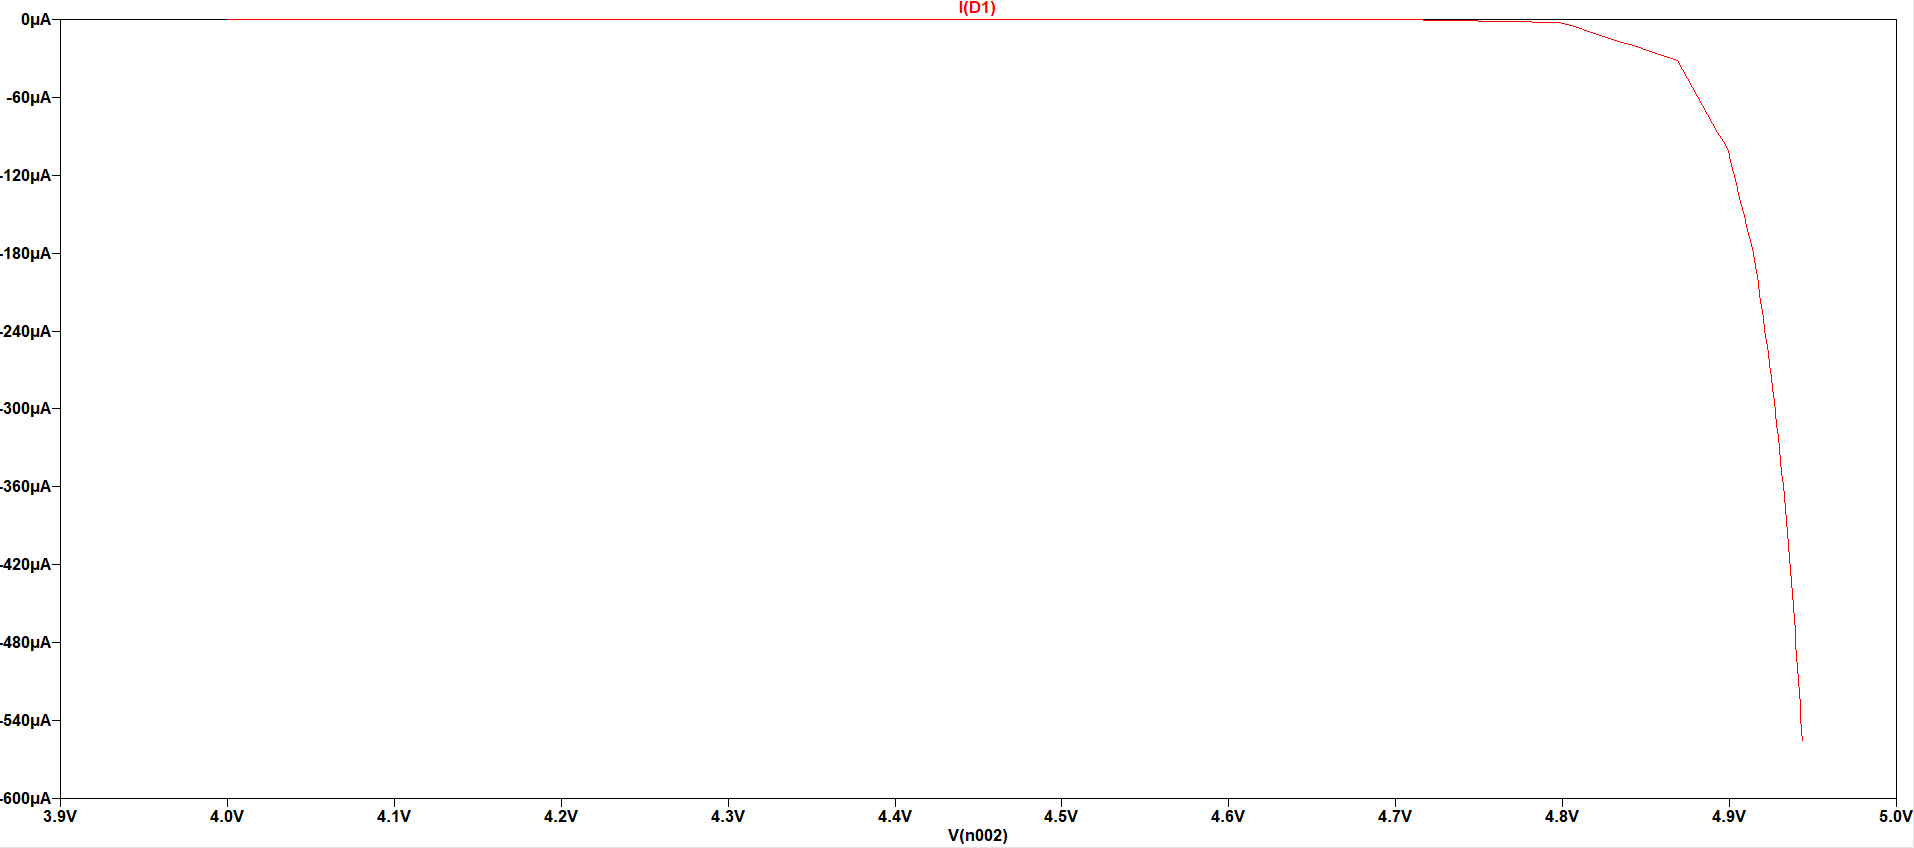
\includegraphics[width=\textwidth]{EXP_1/ZENER_REVERSE/4-5.5v.png}
        \caption{Breakdown Knee ($4\text{ V}$ to $5.5\text{ V}$)}
    \end{subfigure}
    \hfill
    \begin{subfigure}[b]{0.32\textwidth}
        \centering
        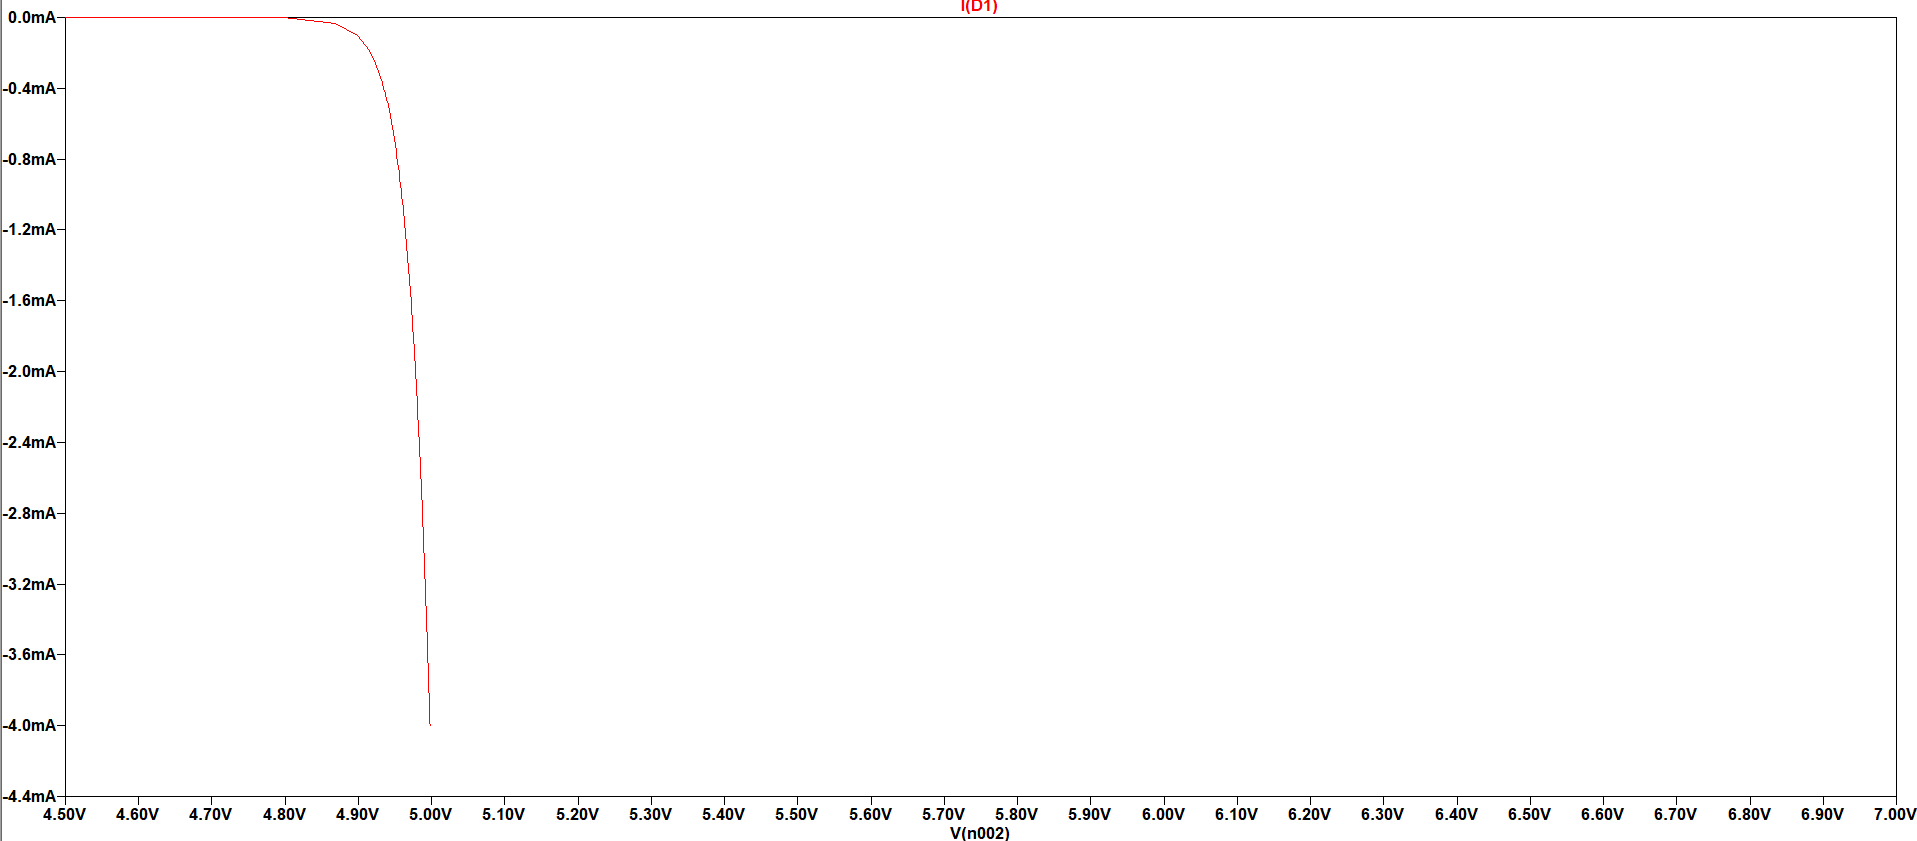
\includegraphics[width=\textwidth]{EXP_1/ZENER_REVERSE/5.5+v.png}
        \caption{Zener Region ($> 5.5\text{ V}$)}
    \end{subfigure}
    \caption{Zener Diode Reverse Breakdown Simulation Response.}
    \label{fig:zener_rev_sim}
\end{figure}

\newpage
\section{Part C: Diode Clipper Circuits}

\subsection{Theoretical Background}
Clippers are wave-shaping circuits that remove portions of an applied signal wave above or below specified reference voltage levels without distorting the remaining part.
\begin{itemize}
    \item \textbf{Positive Clipper:} Clips off the signal waveform above a threshold voltage ($V_{ref} + V_\gamma$).
    \item \textbf{Negative Clipper:} Clips off the signal waveform below a threshold voltage ($-V_{ref} - V_\gamma$).
    \item \textbf{Biased Clipper:} Combines positive and negative clippers to clamp peak amplitudes on both positive and negative half-cycles.
\end{itemize}

\subsection{Circuit Diagrams and Simulation Waveforms}

\subsubsection{Positive Clipper (Clipping above \texorpdfstring{$+1\text{ V}$}{+1V} reference)}
\begin{figure}[H]
    \centering
    \begin{subfigure}[b]{0.48\textwidth}
        \centering
        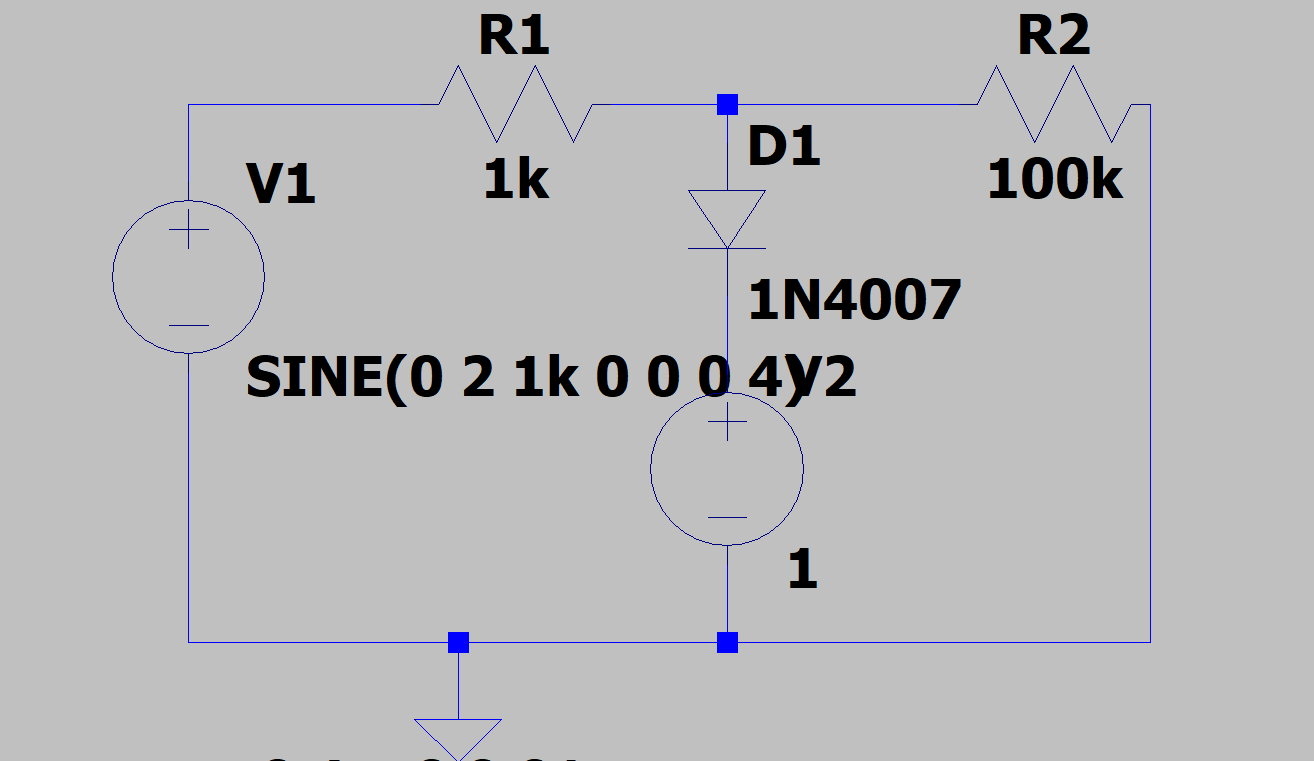
\includegraphics[width=\textwidth]{EXP_1/POSITIVE_CLIPPER/circuit.png}
        \caption{Circuit Diagram}
    \end{subfigure}
    \hfill
    \begin{subfigure}[b]{0.48\textwidth}
        \centering
        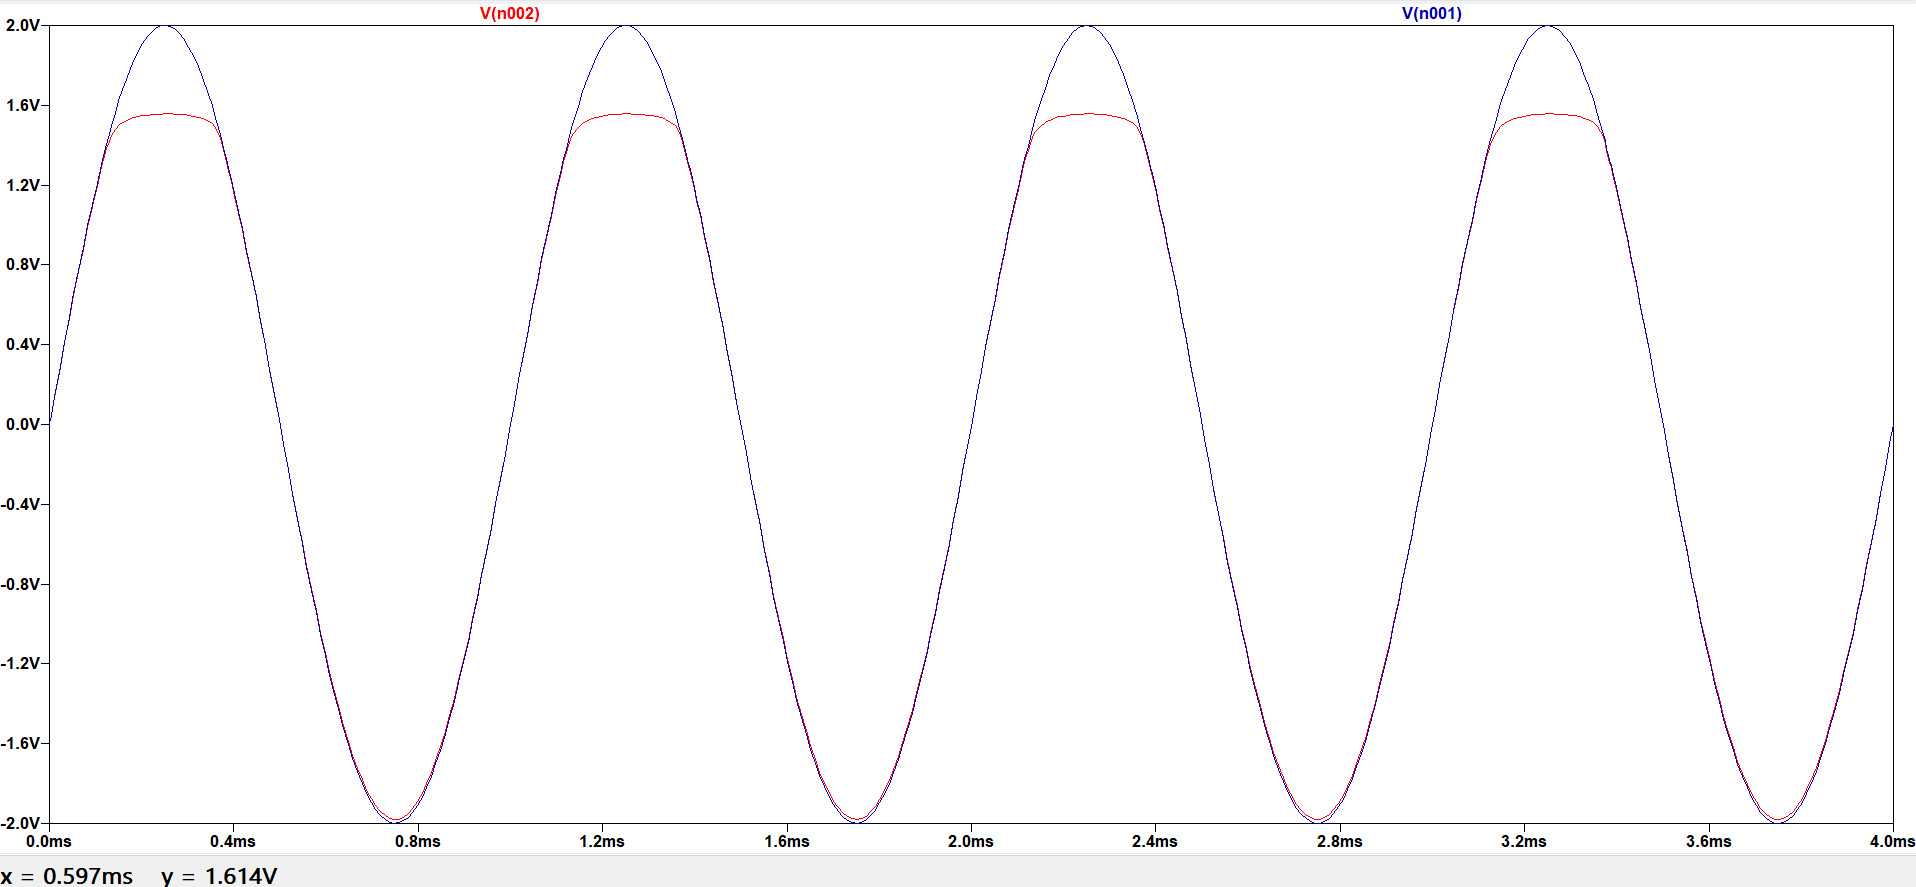
\includegraphics[width=\textwidth]{EXP_1/POSITIVE_CLIPPER/sim.png}
        \caption{Input and Clipped Output Waveforms}
    \end{subfigure}
    \caption{Positive Clipper Circuit and Transient Simulation.}
    \label{fig:pos_clipper}
\end{figure}

\subsubsection{Negative Clipper (Clipping below \texorpdfstring{$-1\text{ V}$}{-1V} reference)}
\begin{figure}[H]
    \centering
    \begin{subfigure}[b]{0.48\textwidth}
        \centering
        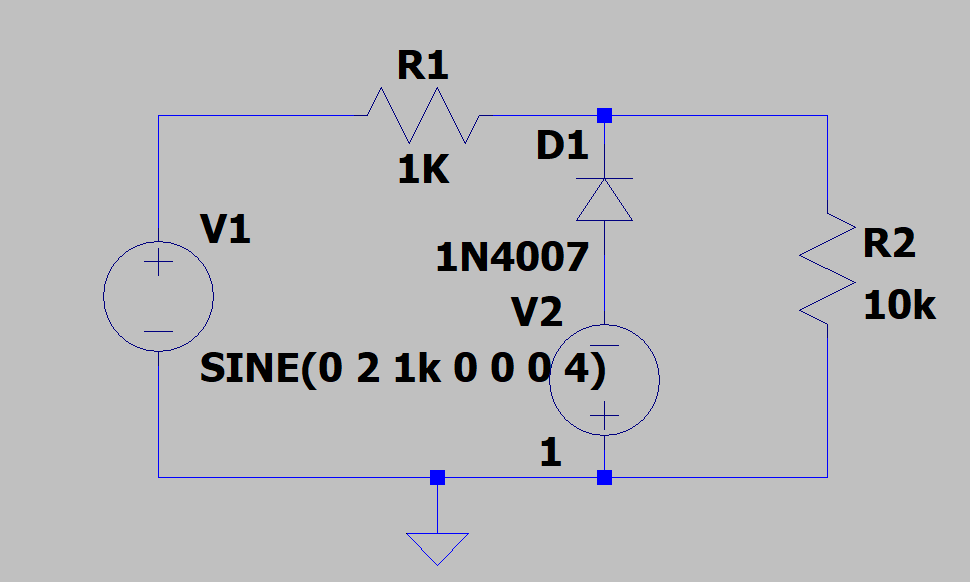
\includegraphics[width=\textwidth]{EXP_1/NEGATIVE_CLIPPER/circuit.png}
        \caption{Circuit Diagram}
    \end{subfigure}
    \hfill
    \begin{subfigure}[b]{0.48\textwidth}
        \centering
        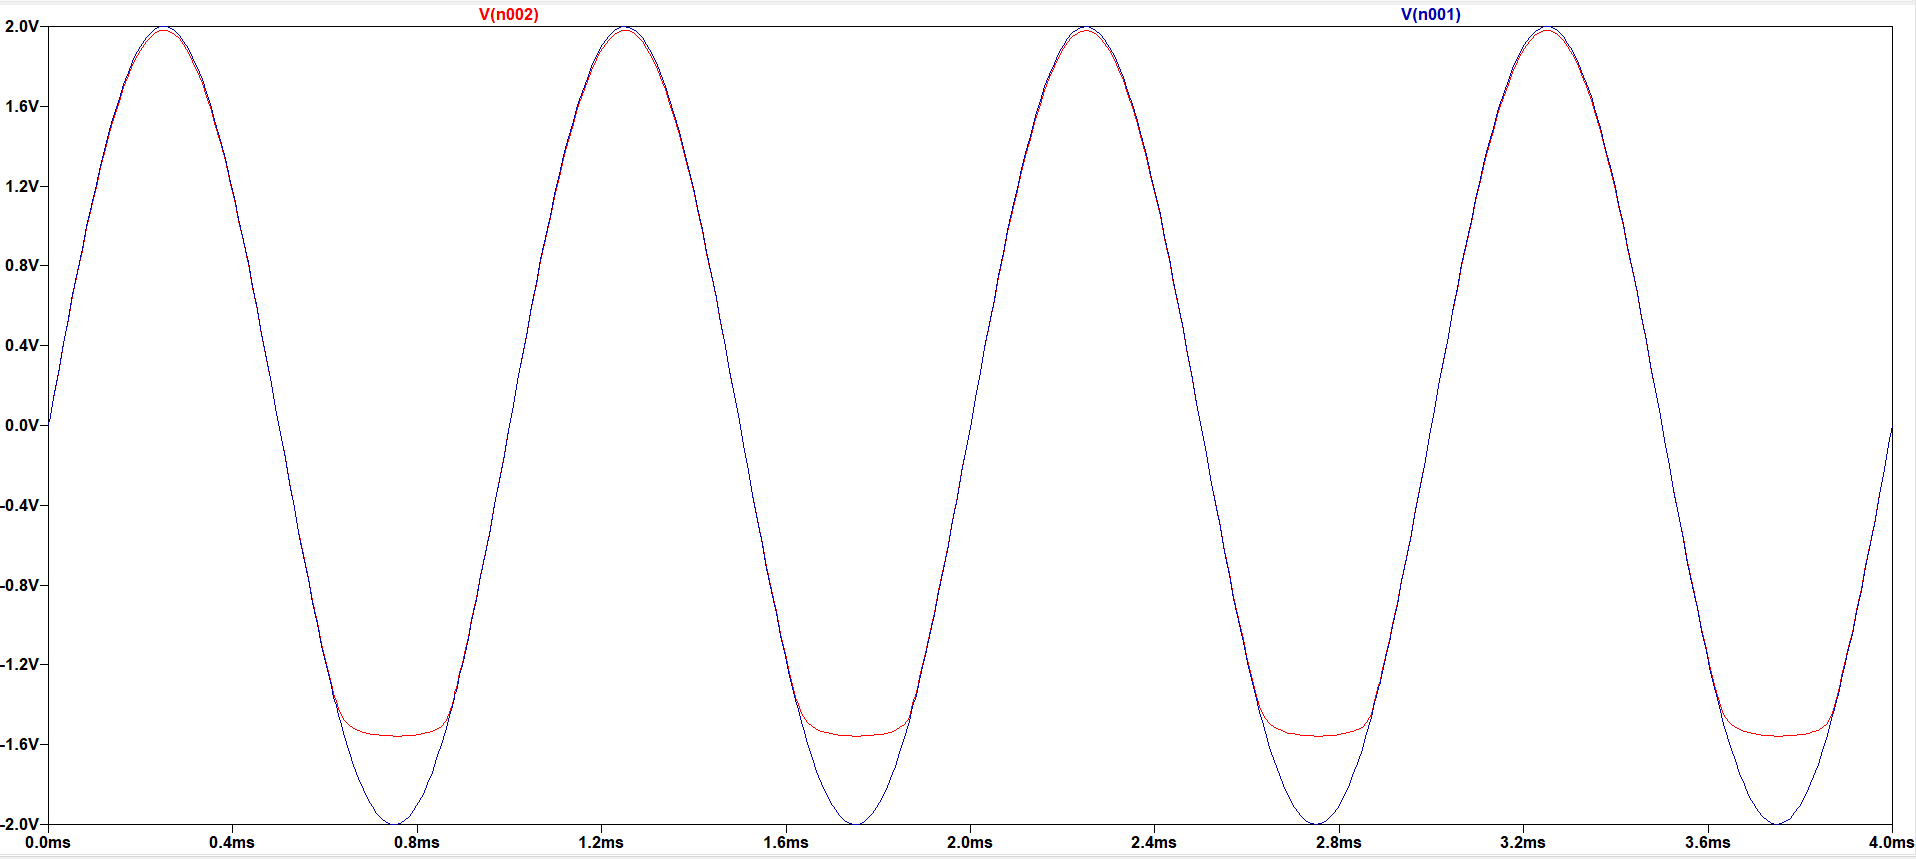
\includegraphics[width=\textwidth]{EXP_1/NEGATIVE_CLIPPER/sim.png}
        \caption{Input and Clipped Output Waveforms}
    \end{subfigure}
    \caption{Negative Clipper Circuit and Transient Simulation.}
    \label{fig:neg_clipper}
\end{figure}

\subsubsection{Biased Clipper (Two-Level Clipper)}
\begin{figure}[H]
    \centering
    \begin{subfigure}[b]{0.48\textwidth}
        \centering
        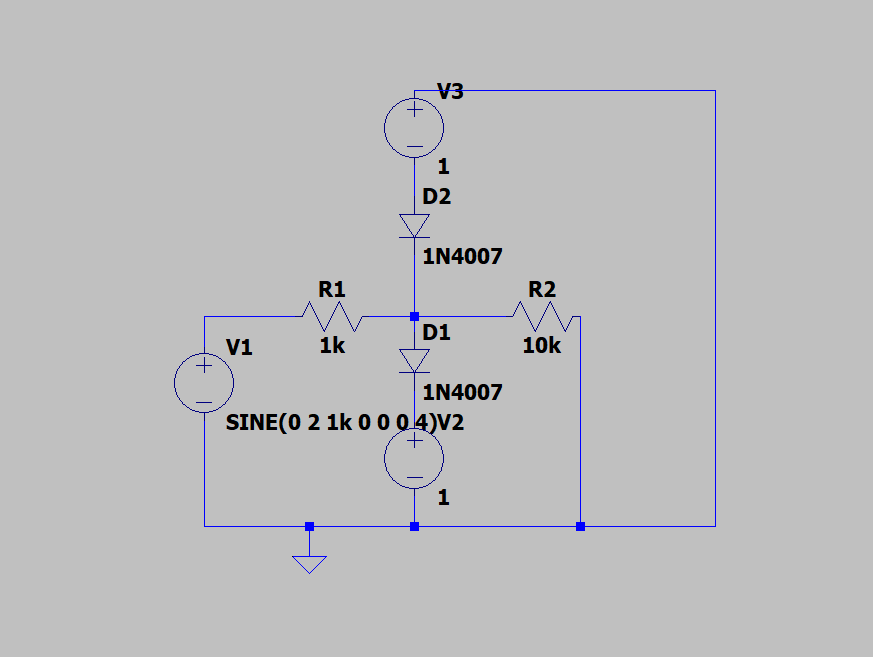
\includegraphics[width=\textwidth]{EXP_1/BIASED_CLIPPER/circuit.png}
        \caption{Circuit Diagram}
    \end{subfigure}
    \hfill
    \begin{subfigure}[b]{0.48\textwidth}
        \centering
        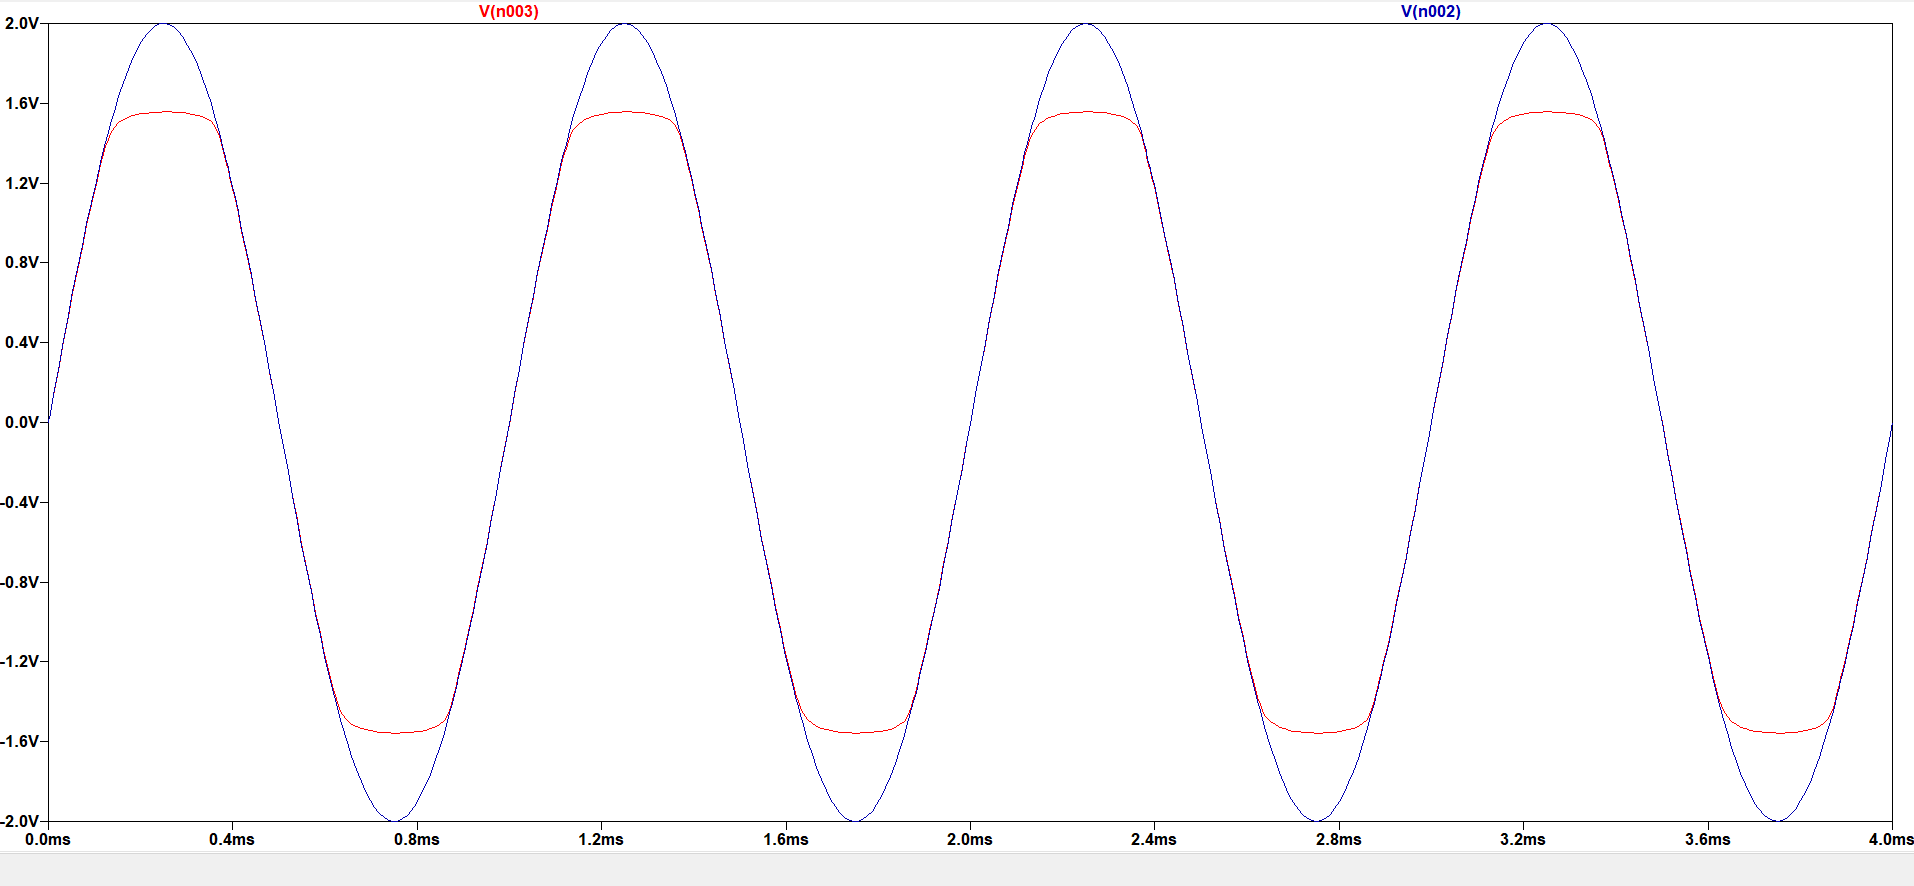
\includegraphics[width=\textwidth]{EXP_1/BIASED_CLIPPER/sim.png}
        \caption{Input and Two-Level Clipped Waveforms}
    \end{subfigure}
    \caption{Biased Clipper Circuit and Transient Simulation.}
    \label{fig:biased_clipper}
\end{figure}

\newpage
\section{Part D: Diode Clamper Circuits}

\subsection{Theoretical Background}
Clampers (DC restorers) shift a waveform vertically by adding a DC level to the input signal without altering the shape or peak-to-peak amplitude of the signal. They consist of a capacitor, diode, and load resistor.
\begin{itemize}
    \item \textbf{Positive Clamper:} Shifts the entire waveform upward so that its minimum peak is clamped near $0\text{ V}$ (or diode drop).
    \item \textbf{Negative Clamper:} Shifts the entire waveform downward so that its maximum peak is clamped near $0\text{ V}$.
\end{itemize}

\subsection{Circuit Diagrams and Simulation Waveforms}

\subsubsection{Positive Clamper}
\begin{figure}[H]
    \centering
    \begin{subfigure}[b]{0.48\textwidth}
        \centering
        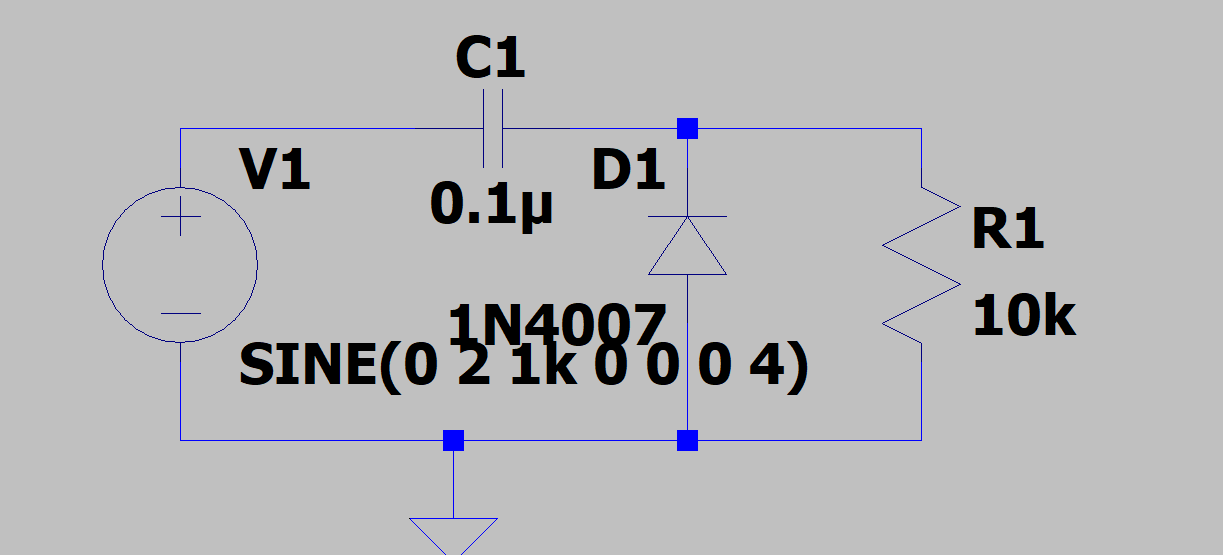
\includegraphics[width=\textwidth]{EXP_1/POSITIVE_CLAMPER/circuit.png}
        \caption{Circuit Diagram}
    \end{subfigure}
    \hfill
    \begin{subfigure}[b]{0.48\textwidth}
        \centering
        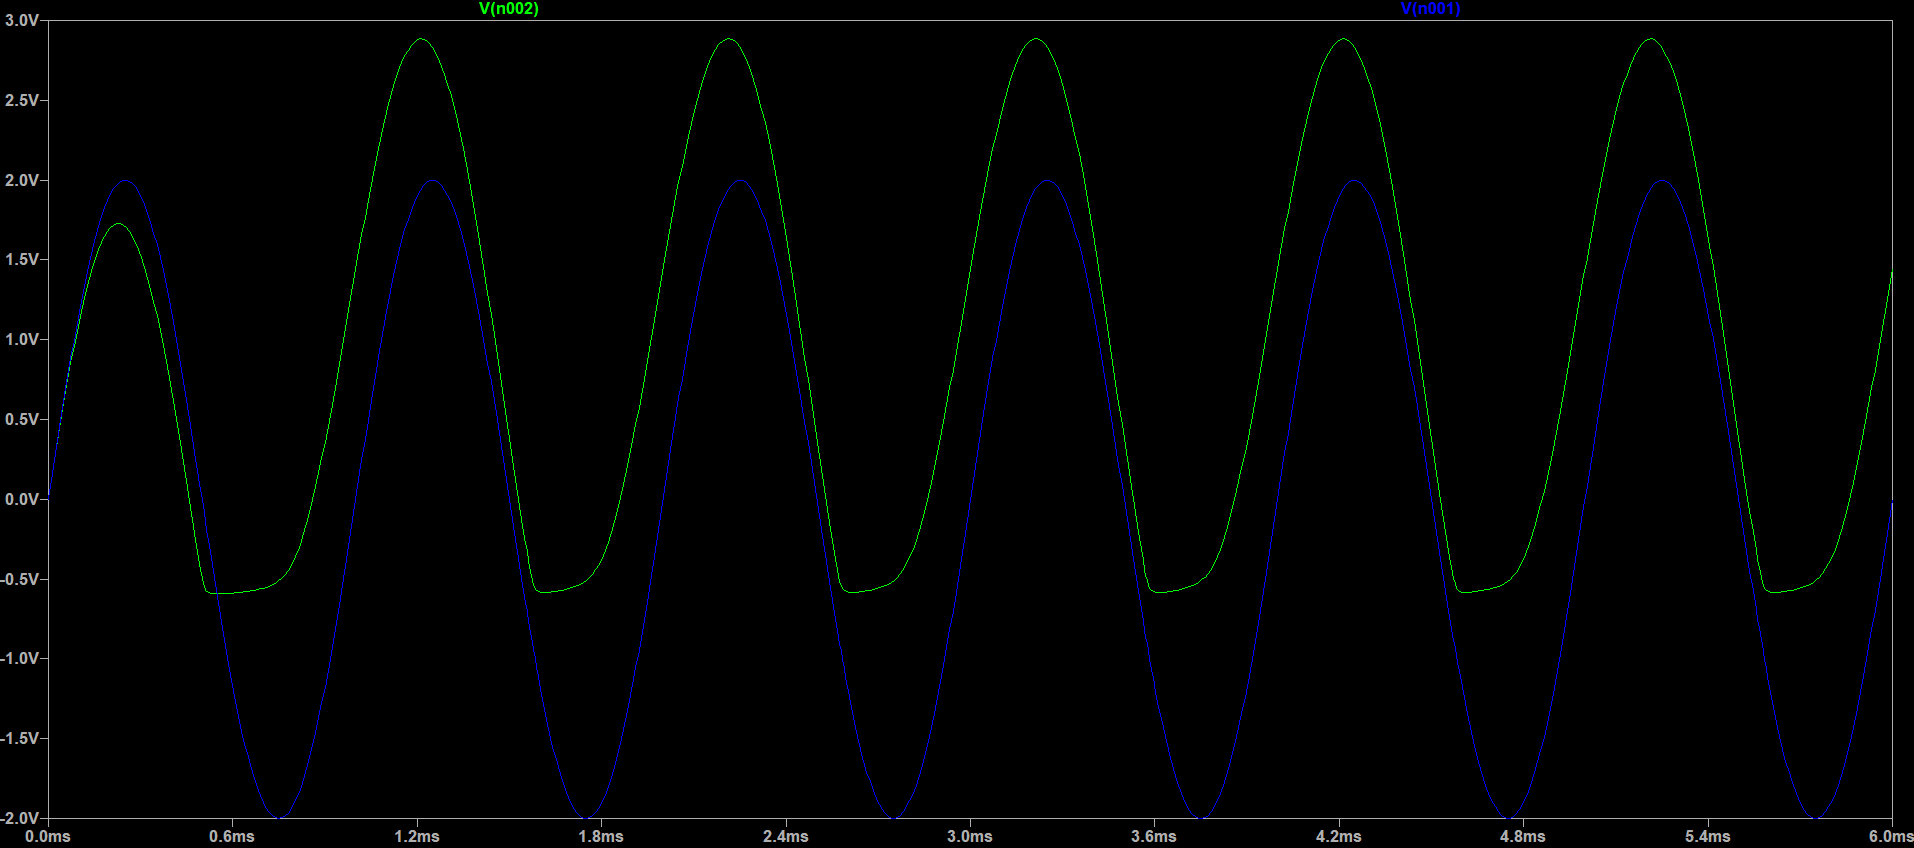
\includegraphics[width=\textwidth]{EXP_1/POSITIVE_CLAMPER/sim.png}
        \caption{Input and Upward Shifted Output Waveforms}
    \end{subfigure}
    \caption{Positive Clamper Circuit and Transient Simulation.}
    \label{fig:pos_clamper}
\end{figure}

\subsubsection{Negative Clamper}
\begin{figure}[H]
    \centering
    \begin{subfigure}[b]{0.48\textwidth}
        \centering
        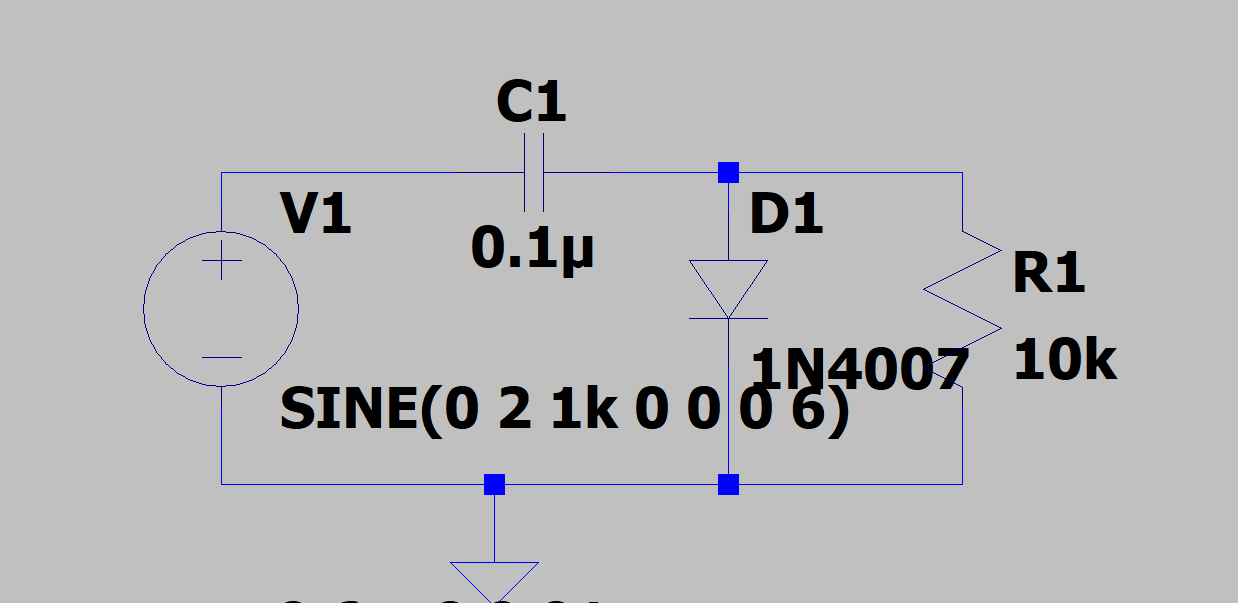
\includegraphics[width=\textwidth]{EXP_1/NEGATIVE_CLAMPER/circuit.png}
        \caption{Circuit Diagram}
    \end{subfigure}
    \hfill
    \begin{subfigure}[b]{0.48\textwidth}
        \centering
        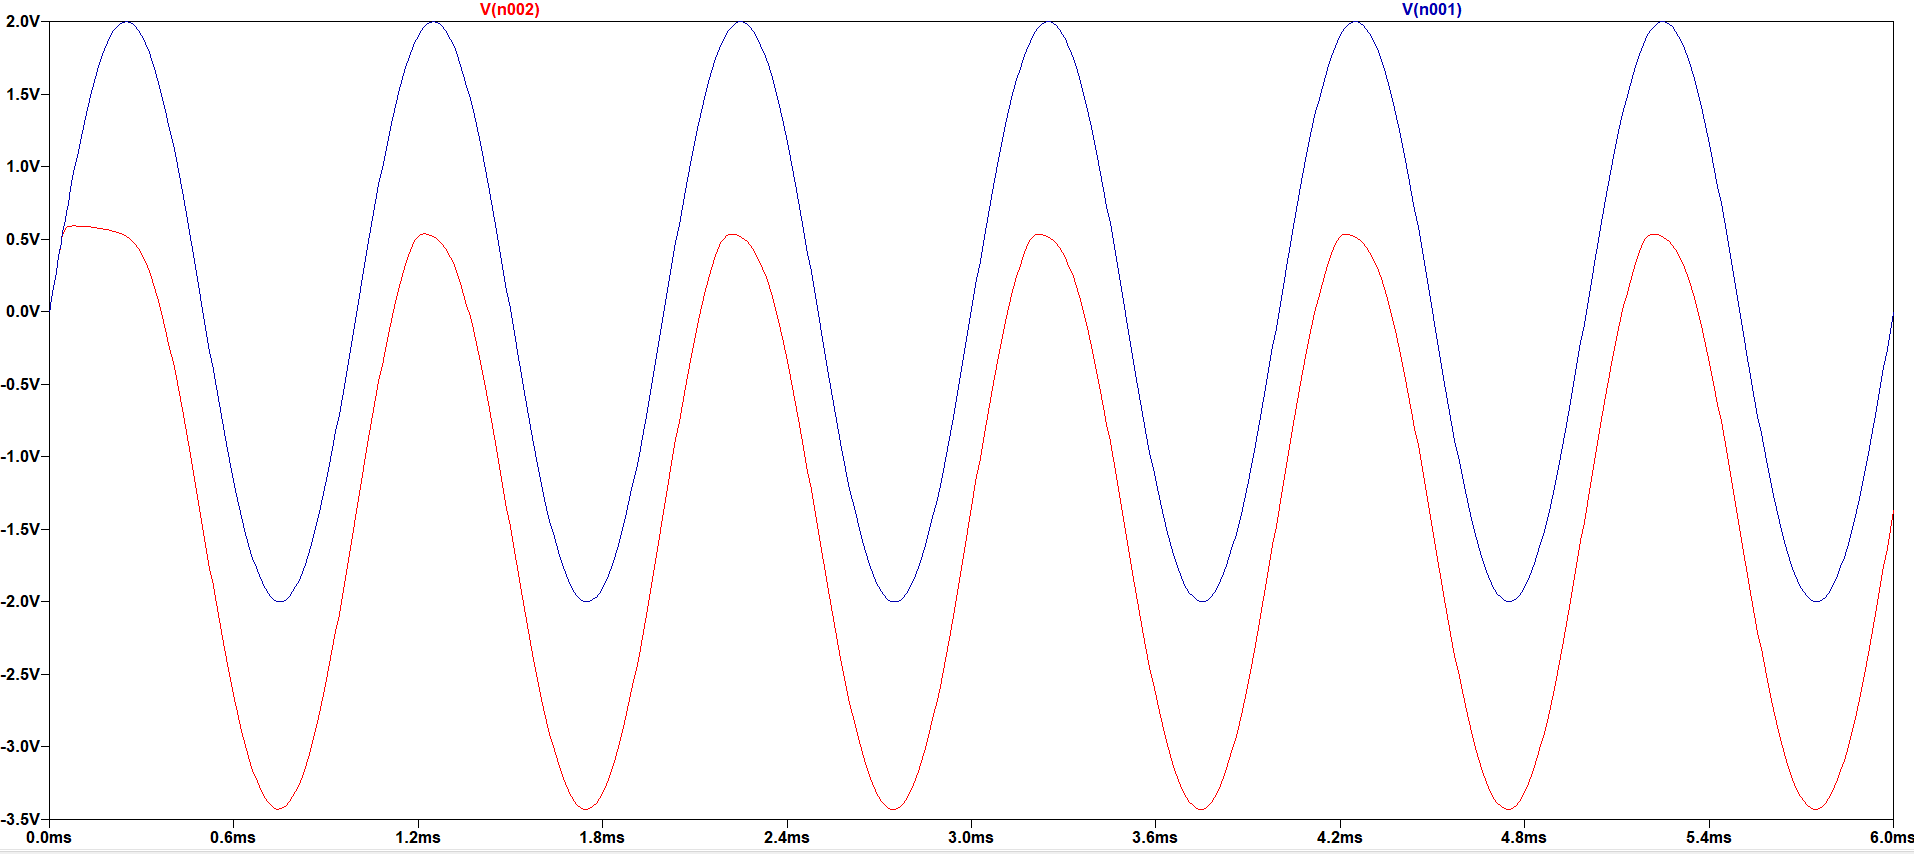
\includegraphics[width=\textwidth]{EXP_1/NEGATIVE_CLAMPER/sim.png}
        \caption{Input and Downward Shifted Output Waveforms}
    \end{subfigure}
    \caption{Negative Clamper Circuit and Transient Simulation.}
    \label{fig:neg_clamper}
\end{figure}

\section{Observation Tables (Experimental Data Placeholder)}
\textit{Note: Experimental readings to be populated post hardware testing.}

\subsection{Forward and Reverse Bias Observations}
\begin{table}[H]
\centering
\caption{PN Junction Diode and Zener Diode Conduction Data}
\begin{tabular}{c c c | c c c}
\toprule
\multicolumn{3}{c|}{\textbf{PN Junction Diode (1N4007)}} & \multicolumn{3}{c}{\textbf{Zener Diode (1N4733A)}} \\
\midrule
\textbf{S.No.} & \textbf{$V_f$ (V)} & \textbf{$I_f$ (mA)} & \textbf{S.No.} & \textbf{$V_r$ (V)} & \textbf{$I_r$ (mA)} \\
\midrule
1 & & & 1 & & \\
2 & & & 2 & & \\
3 & & & 3 & & \\
4 & & & 4 & & \\
5 & & & 5 & & \\
6 & & & 6 & & \\
7 & & & 7 & & \\
8 & & & 8 & & \\
\bottomrule
\end{tabular}
\end{table}

\subsection{Clipper and Clamper Summary Table}
\begin{table}[H]
\centering
\caption{Wave-shaping Circuits Performance Summary}
\begin{tabular}{l c c c}
\toprule
\textbf{Circuit} & \textbf{Input $V_{pp}$ (V)} & \textbf{Theoretical Threshold/Shift} & \textbf{Measured Output Level} \\
\midrule
Positive Clipper & 4.0 & $+1.0\text{ V} + V_\gamma$ & \\
Negative Clipper & 4.0 & $-1.0\text{ V} - V_\gamma$ & \\
Biased Clipper   & 4.0 & $+1.0\text{ V}$ and $-1.0\text{ V}$ limits & \\
Positive Clamper & 4.0 & $+V_p - V_\gamma \approx +1.3\text{ V}$ shift & \\
Negative Clamper & 4.0 & $-V_p + V_\gamma \approx -1.3\text{ V}$ shift & \\
\bottomrule
\end{tabular}
\end{table}

\section{Conclusion}
The simulation and theoretical study for Experiment 1 were successfully performed. The forward and reverse characteristics of both the standard PN diode and the Zener diode match theoretical expectations. Furthermore, the transient response of the positive, negative, and biased clipper circuits as well as the positive and negative clamper circuits demonstrate accurate signal shaping and DC level restoration.

\end{document}
